\appendix
\renewcommand{\cftchappresnum}{Appendix }
\chapter{PCB Schematics}
%\addcontentsline{toc}{chapter}{ WHIP Schematics }
\label{chap:PCB_Schematics}
\begin{figure}
	\begin{center}
		\label{fig:FullSchematic_Sheet1}
		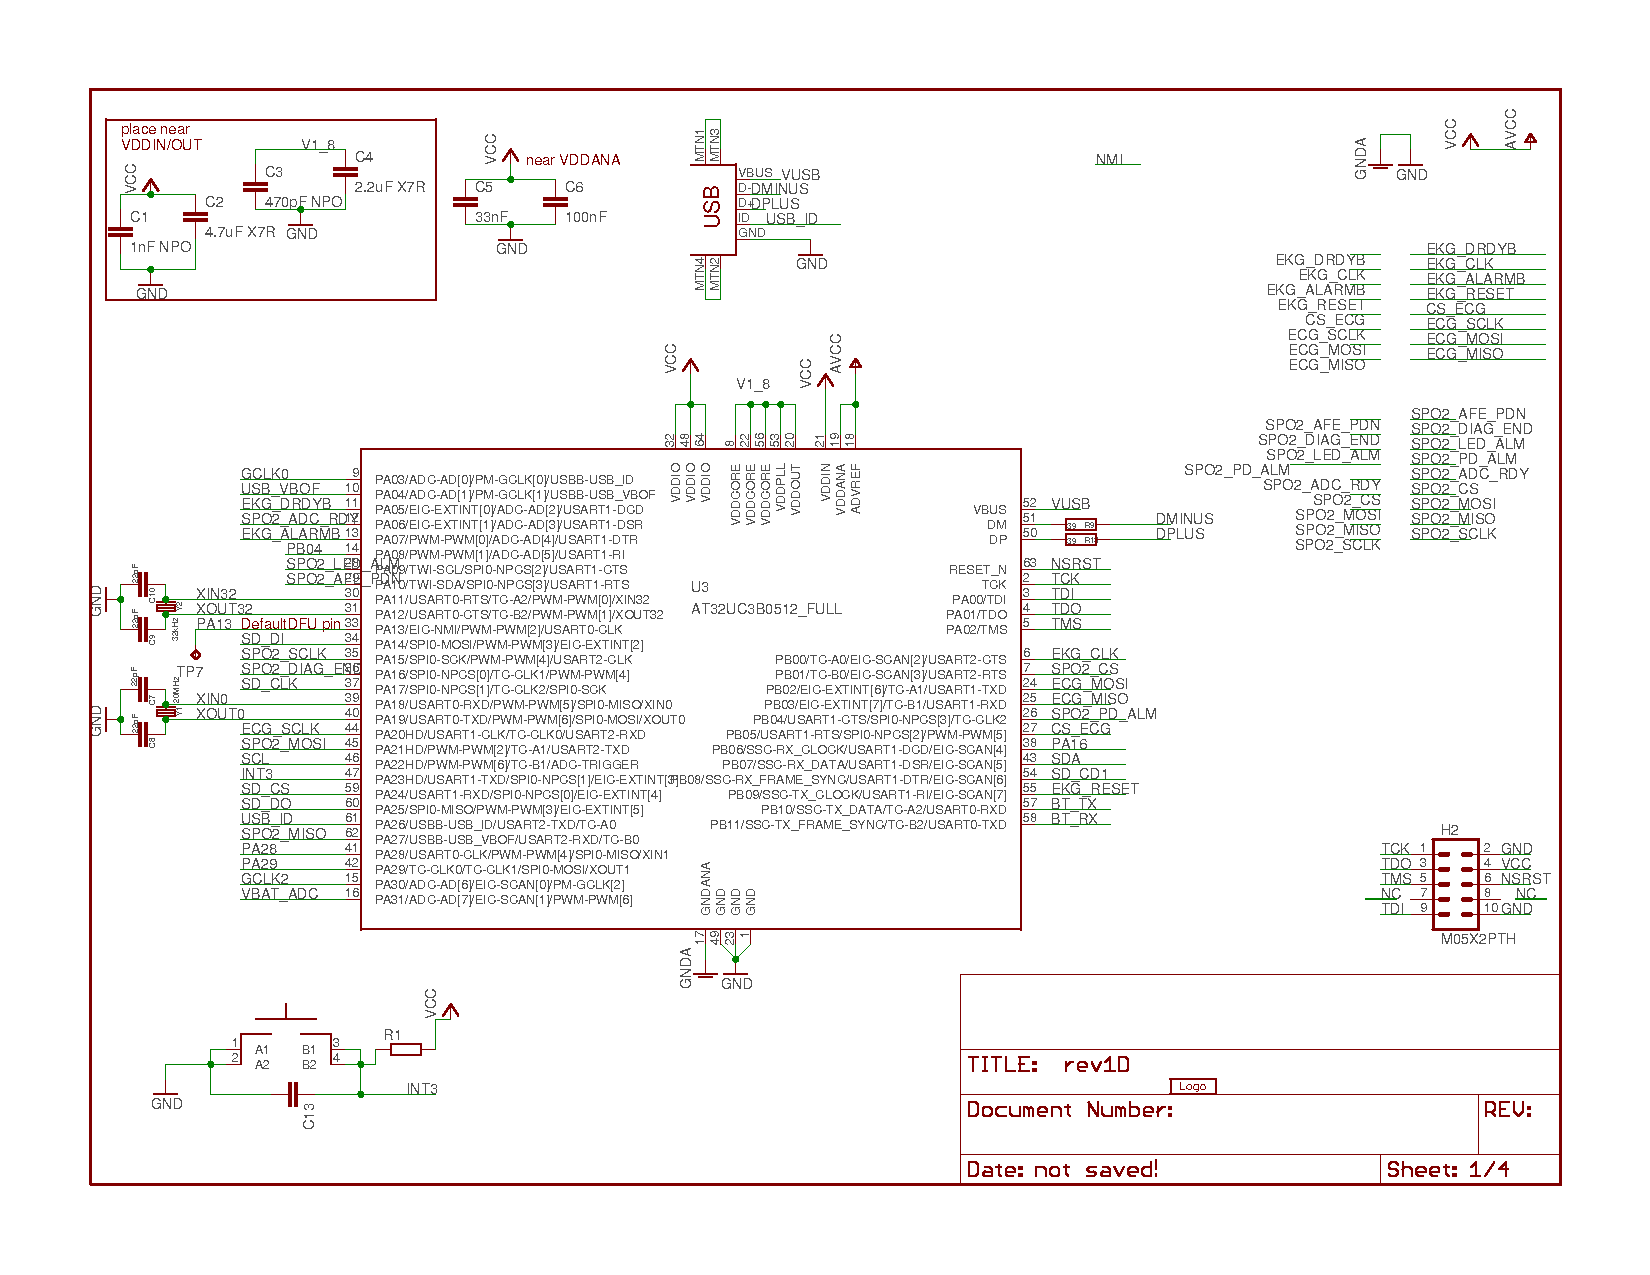
\includegraphics[angle=90,scale=1,width=1\textwidth]{Images/rev1D_sheet1.pdf} 
		\caption{Full Schematic, Microprocessor View}
	\end{center}
\end{figure}

\begin{figure}
	\begin{center}
		\label{fig:FullSchematic_Sheet2}
		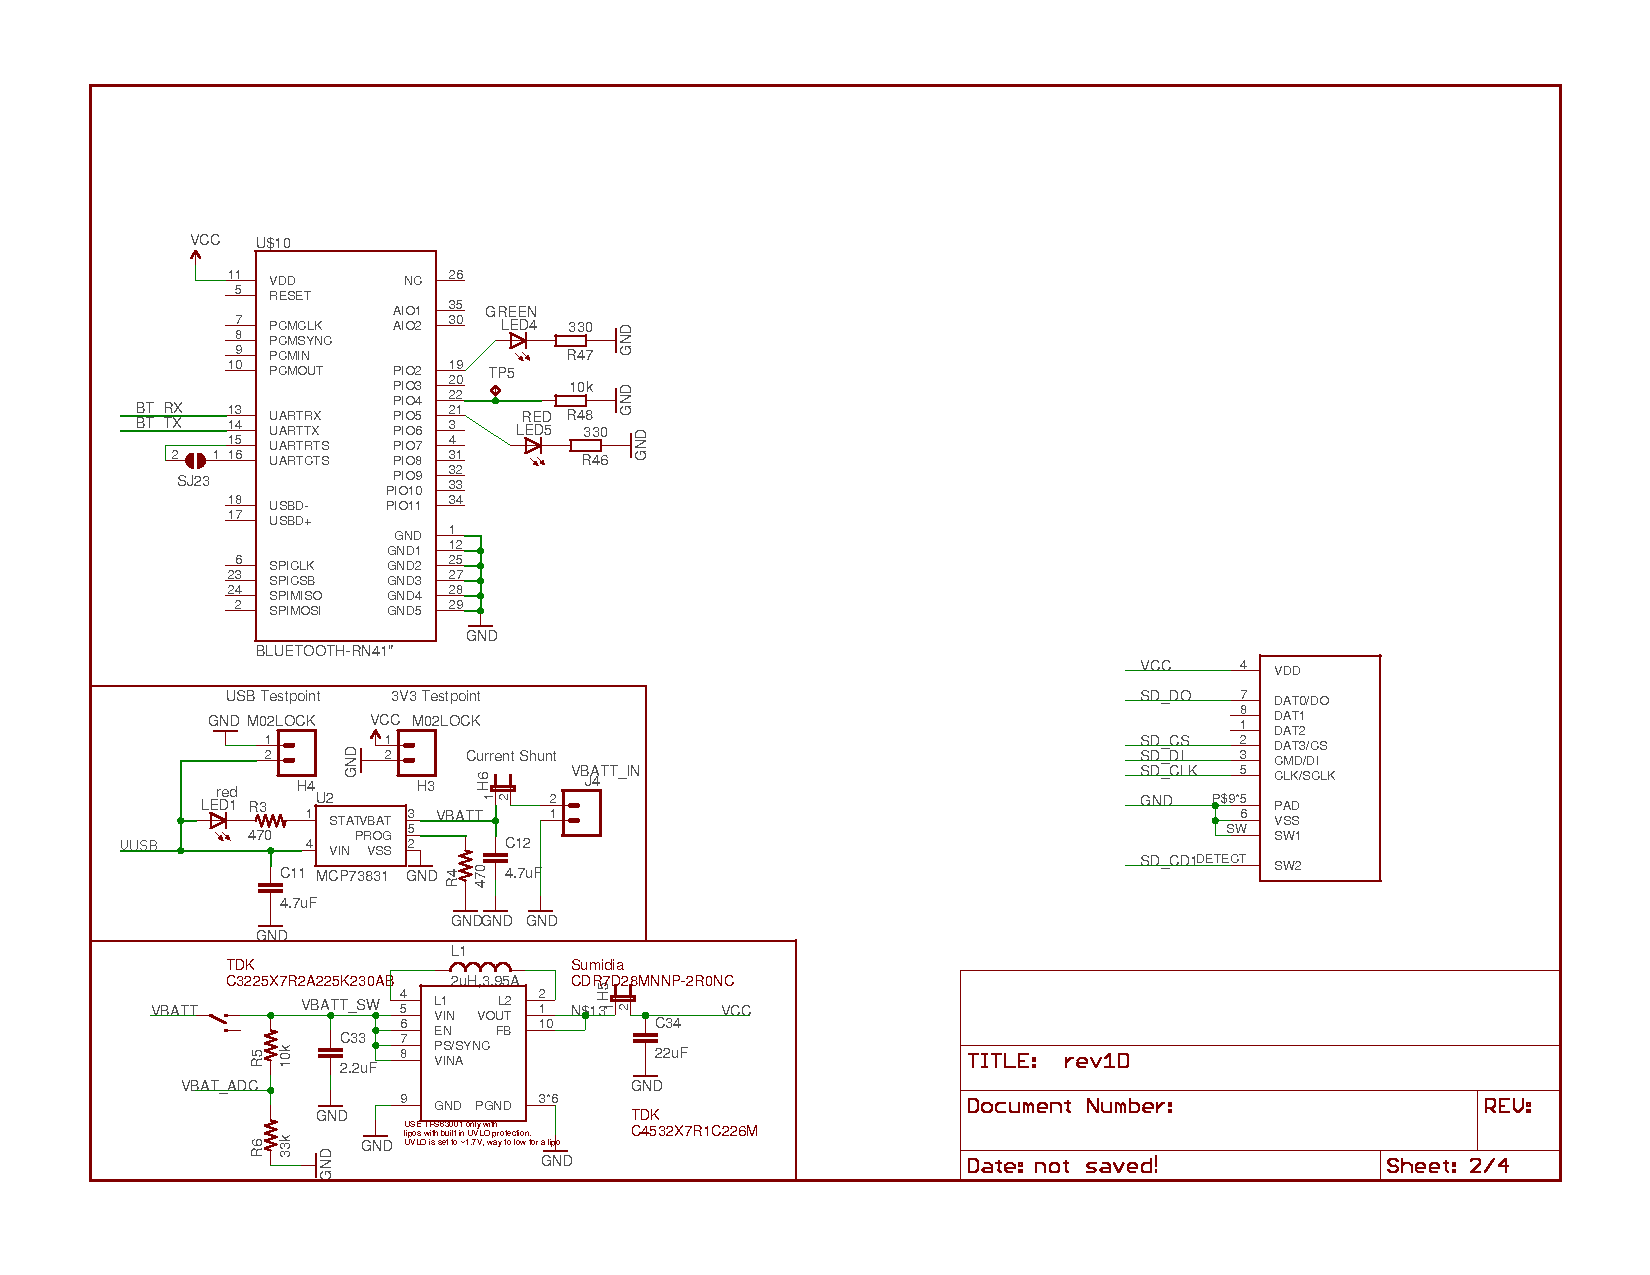
\includegraphics[angle=90,scale=1,width=1\textwidth]{Images/rev1D_sheet2.pdf} 
		\caption{Full Schematic, Bluetooth, Power System, and SD Card View}
	\end{center}
\end{figure}

\begin{figure}
	\begin{center}
		\label{fig:FullSchematic_Sheet3}
		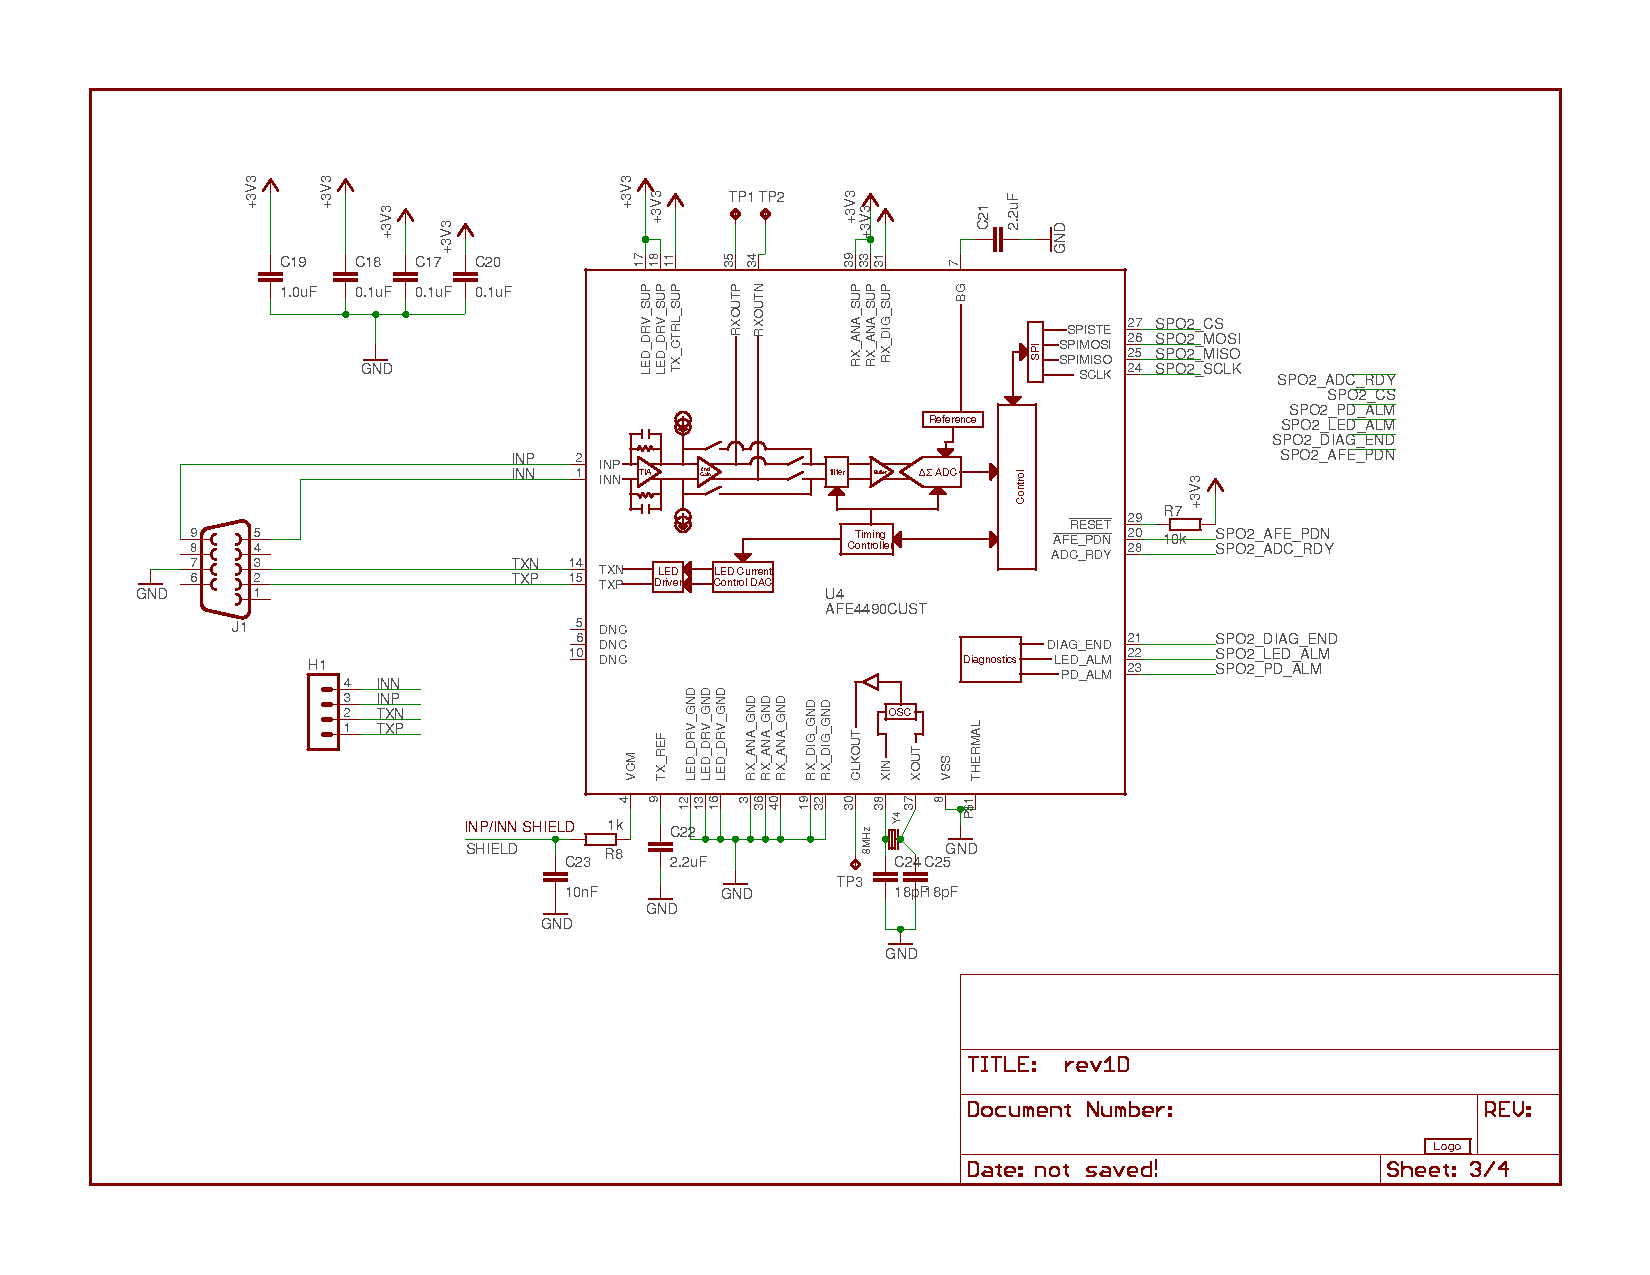
\includegraphics[angle=90,scale=1,width=1\textwidth]{Images/rev1D_sheet3.pdf} 
		\caption{Full Schematic, \spo2 View}
	\end{center}
\end{figure}

\begin{figure}
	\begin{center}
		\label{fig:FullSchematic_Sheet4}
		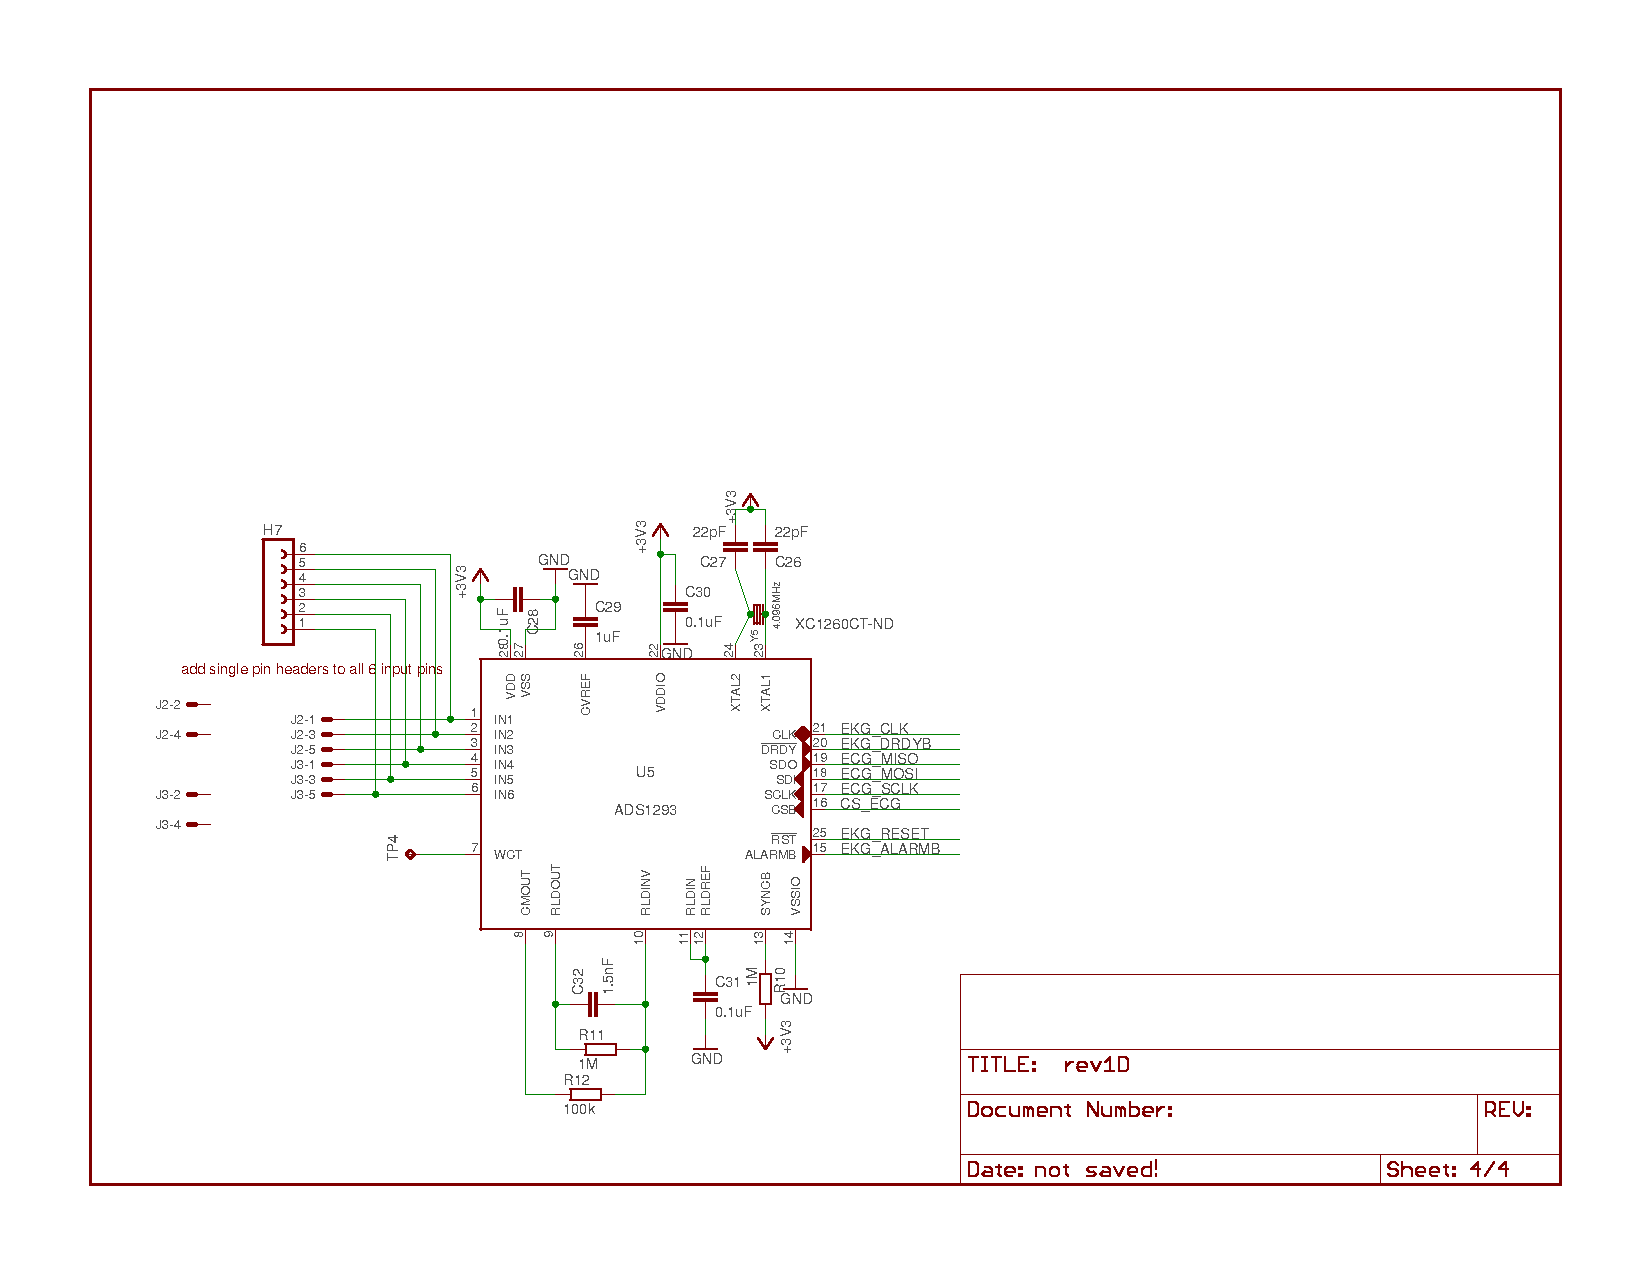
\includegraphics[angle=90,scale=1,width=1\textwidth]{Images/rev1D_sheet4.pdf} 
		\caption{Full Schematic ECG View}
	\end{center}
\end{figure}

\chapter{PCB LAYOUT}
%\addcontentsline{toc}{chapter}{ WHIP Layout }
\label{chap:PCB_LAYOUT}

\begin{figure}
\begin{center}
	\label{fig:TOPGerber}
	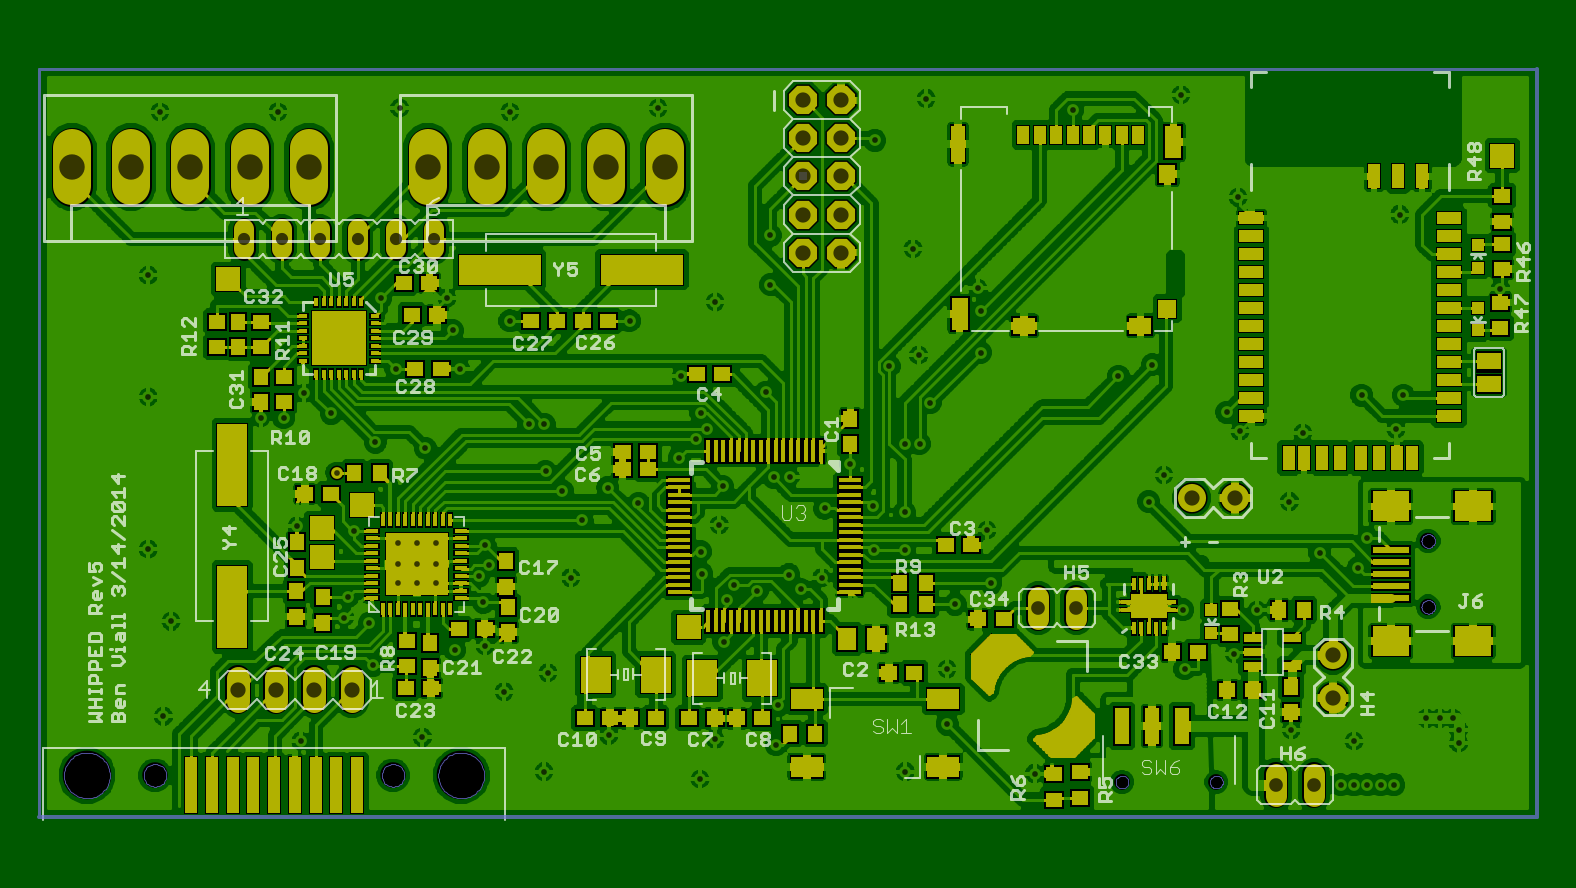
\includegraphics[angle=0,scale=1,width=1\textwidth]{Images/Rev5_TOPGERB.png} 
	\caption{Gerber Render for Top Layer}
\end{center}
\end{figure}


\begin{figure}
\begin{center}
	\label{fig:BOTGerber}
	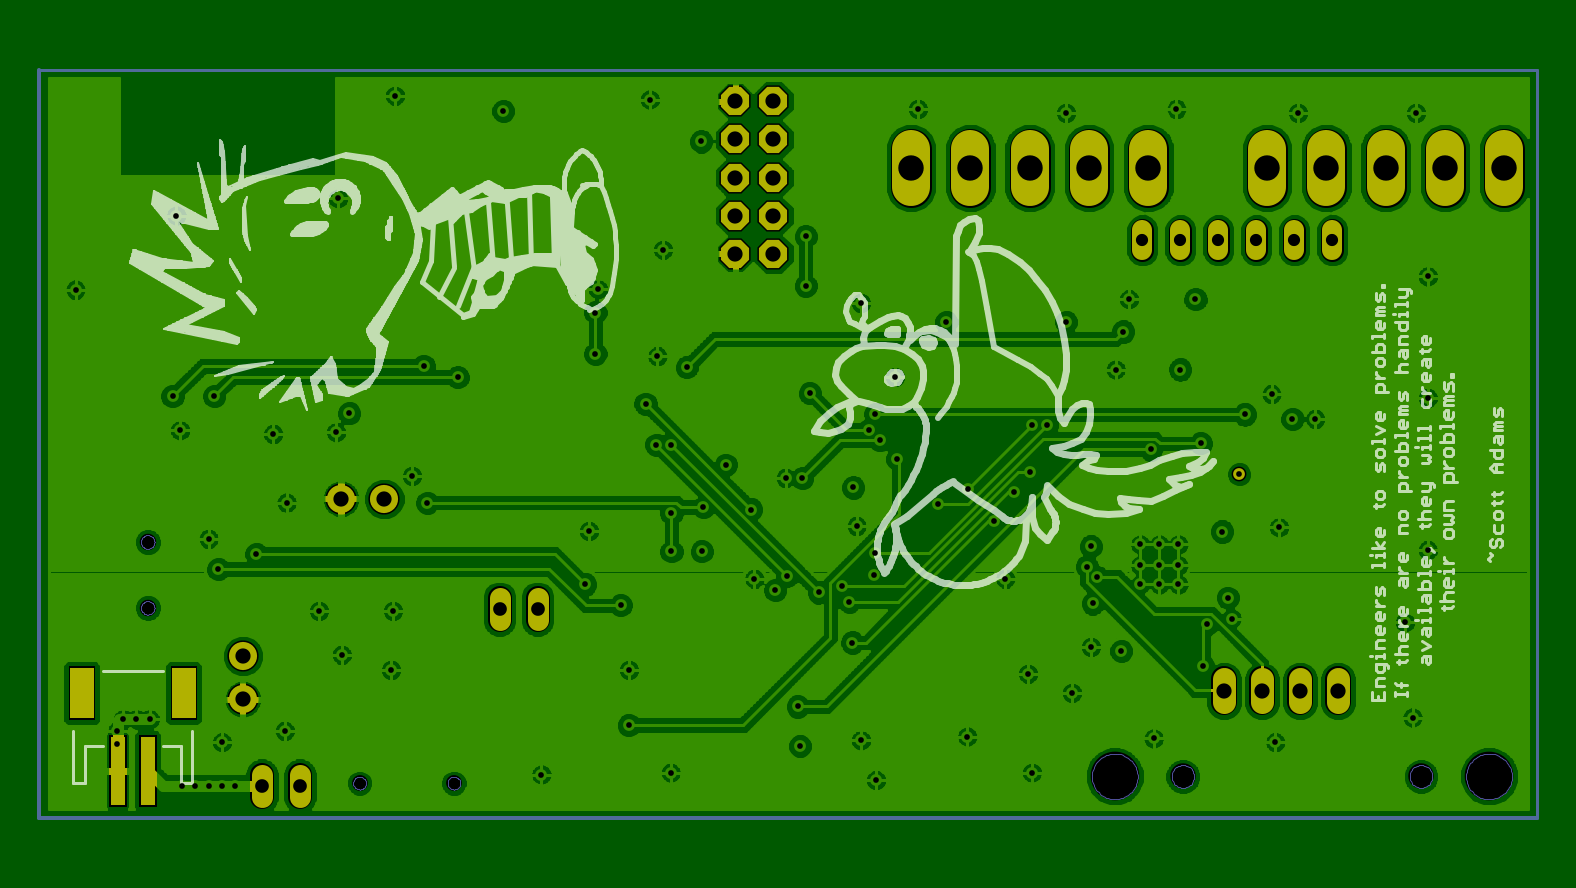
\includegraphics[angle=0,scale=1,width=1\textwidth]{Images/Rev5_BOTGERB.png} 
	\caption{Gerber Render for Bottom Layer}
\end{center}
\end{figure}


\begin{figure}
\begin{center}
	\label{fig:GNDGerber}
	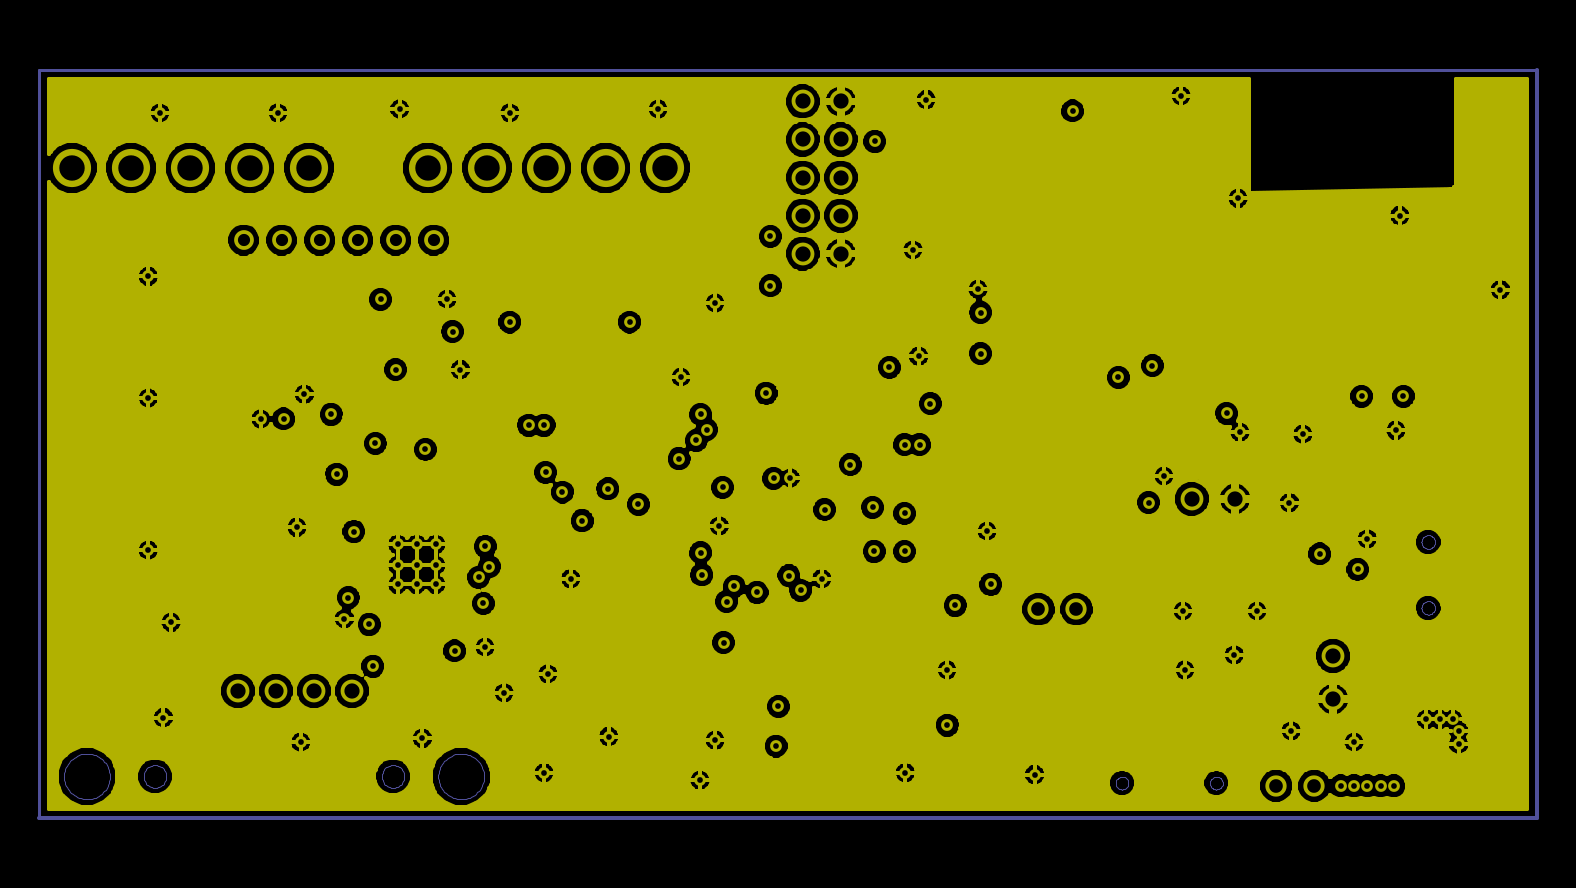
\includegraphics[angle=0,scale=1,width=1\textwidth]{Images/Rev5_GNDGERB.png} 
	\caption{Gerber Render for Internal Ground Layer}
\end{center}
\end{figure}


\begin{figure}
\begin{center}
	\label{fig:PWRGerber}
	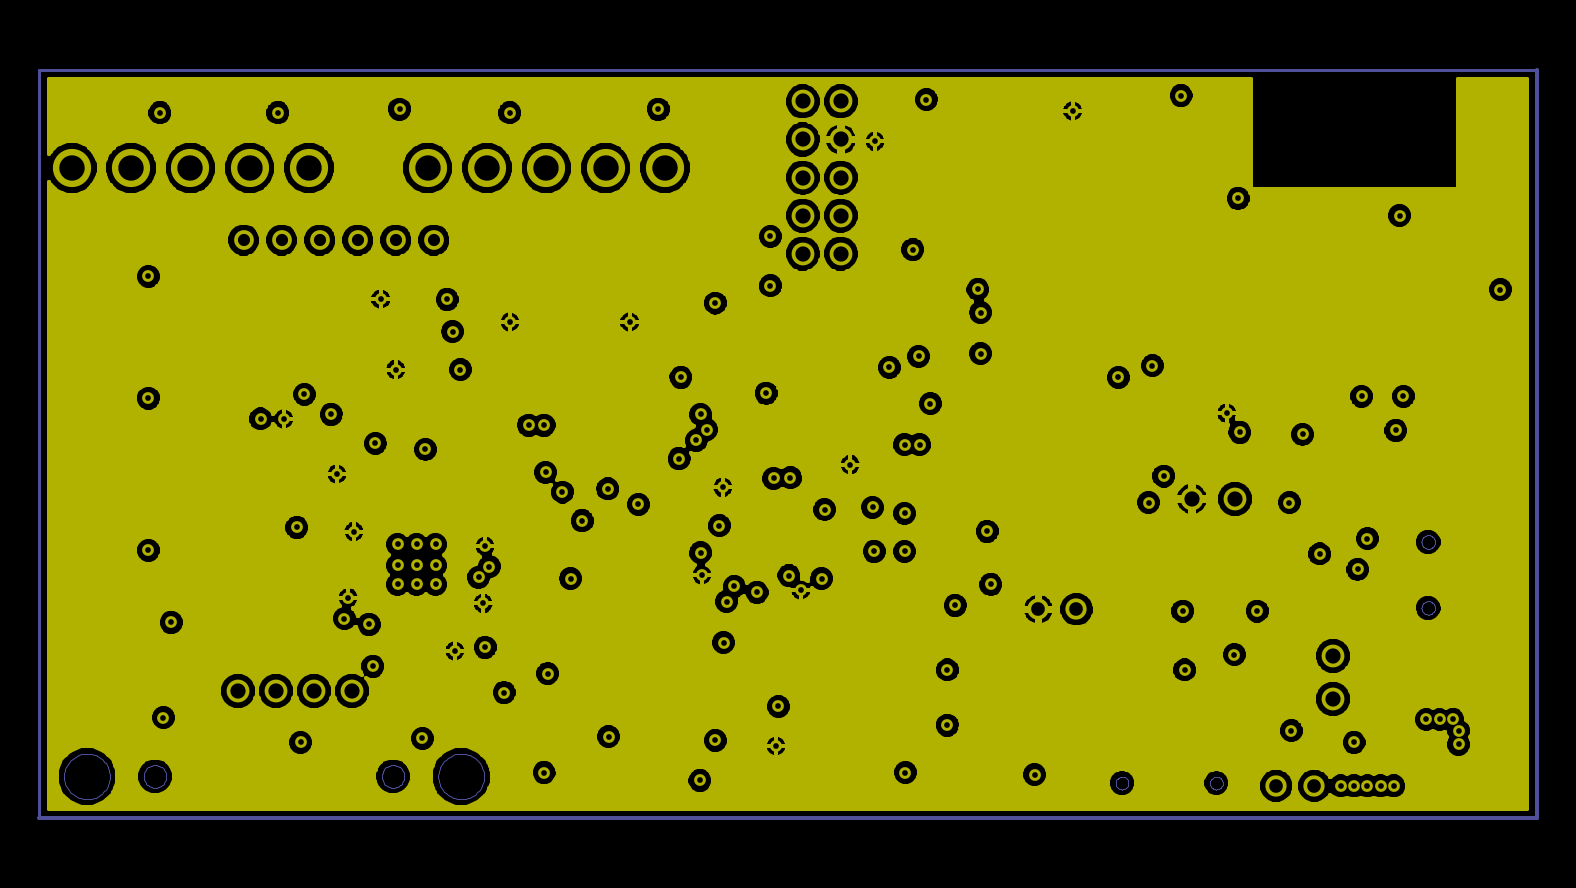
\includegraphics[angle=0,scale=1,width=1\textwidth]{Images/Rev5_PWRGERB.png} 
	\caption{Gerber Render for Internal Power Layer}
\end{center}
\end{figure}
